\section*{A-3. データ収集から特徴量抽出(使用モデルは4章にしたい)}
この章では,BLEを用いた混雑度推定手法について述べる.

\subsection*{3.1 BLEスキャンと正解ラベルの取得}
この章では,学生食堂内のBLEデータと,その時点の食堂利用人数の計測方法を述べる.

\subsubsection*{Rasberry PiによるBLEスキャン}
BLEスキャンは図\ref{raspi}のようなRaspberry Piを用いて行う.
スキャンは約10秒の間隔で行われ,1回のスキャンに含まれる情報は以下の通りである.
\begin{itemize}
  \item BLE情報(MACアドレス,RSSI)
  \item スキャン時刻
\end{itemize}

\begin{figure}[pt]
  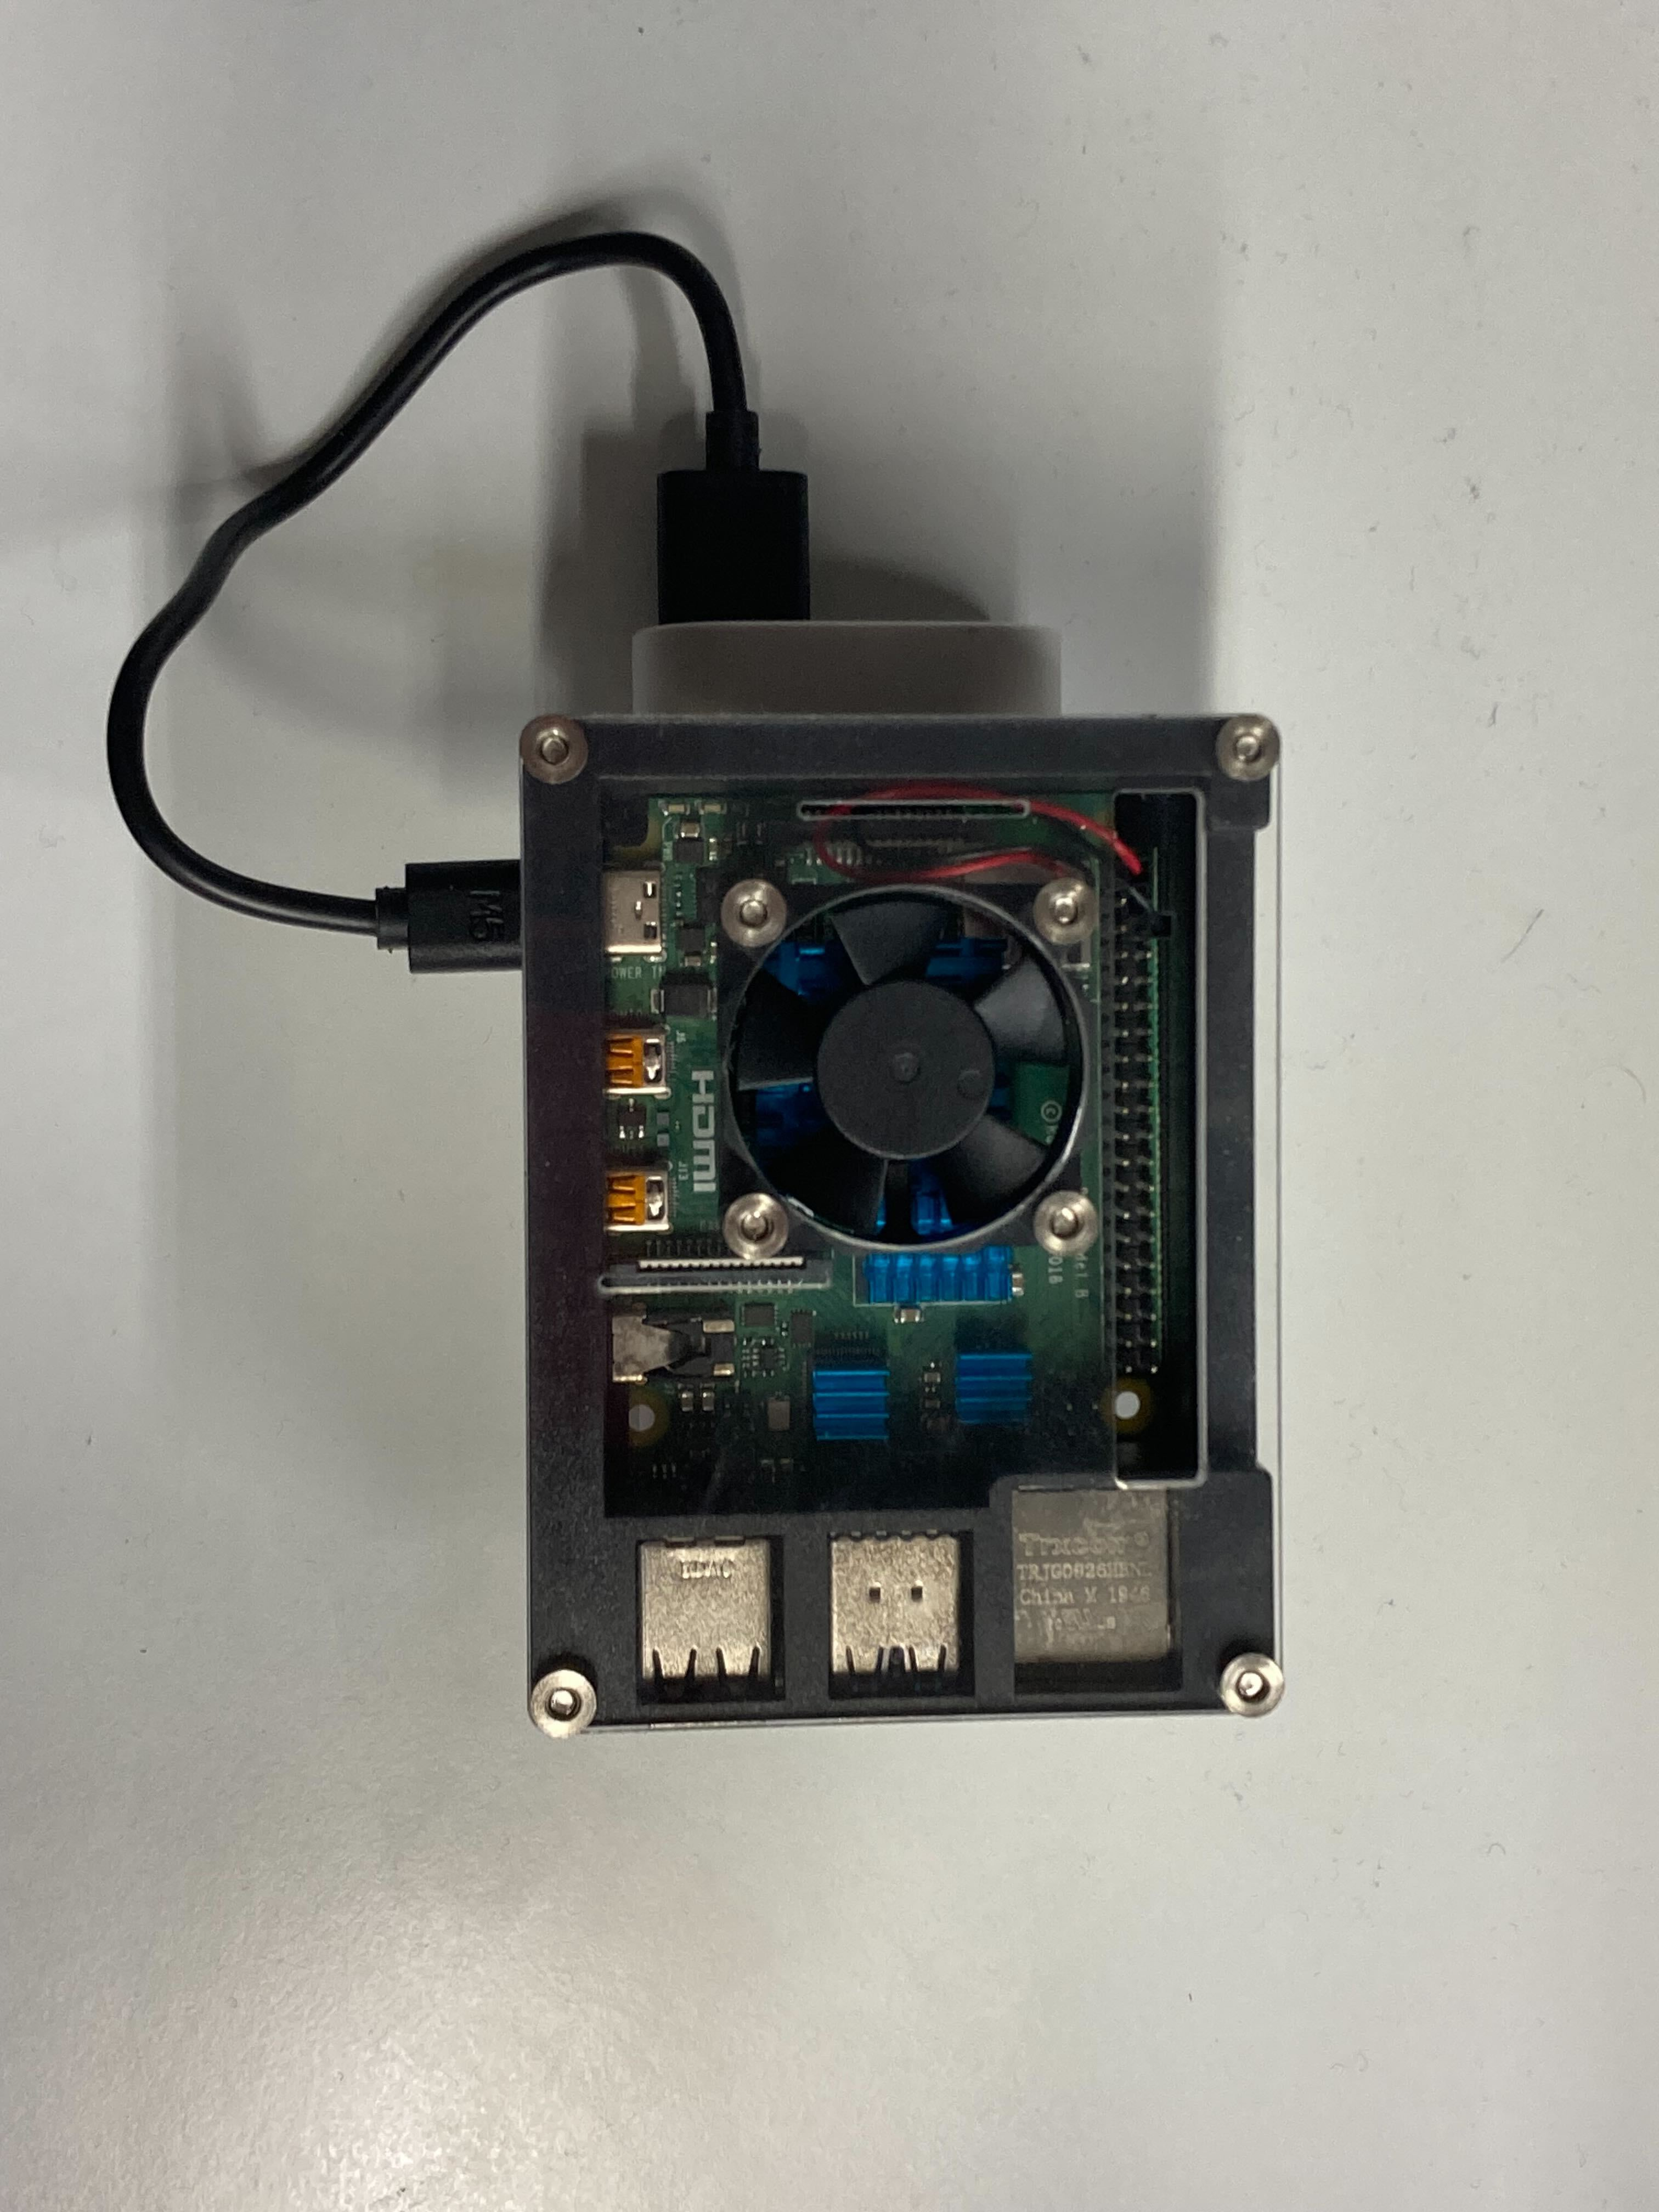
\includegraphics[scale=0.07]{./images/raspi.jpg}
  \centering
  \caption{設置したRasberry Pi\label{raspi}}
\end{figure}

図\ref{raspi_place}に学生食堂の概略図とRasberry Piの設置位置を示す.
基本的に壁などの空間を隔てるような障害物は存在せず,開けた空間となっており,そこに机や椅子が配置されている.
Rasberry Piは学生食堂1階と2階それぞれのフロアの中央に計2台配置する.
それぞれのRasberry Piはお互いに異なるタイミングでスキャンを開始するため,
2台のRasberry Piは同期していない.
Rasberry Piは1階と2階に配置するが,1階と2階は完全に別の空間ではなく,
スキャン範囲が重複していることに注意が必要である.
そのため,あえて同期を取らないことで,違うタイミングでスキャンが行われ,
BLEデータの時間方向における分解能を向上させることができる.
\begin{figure}[pt]
  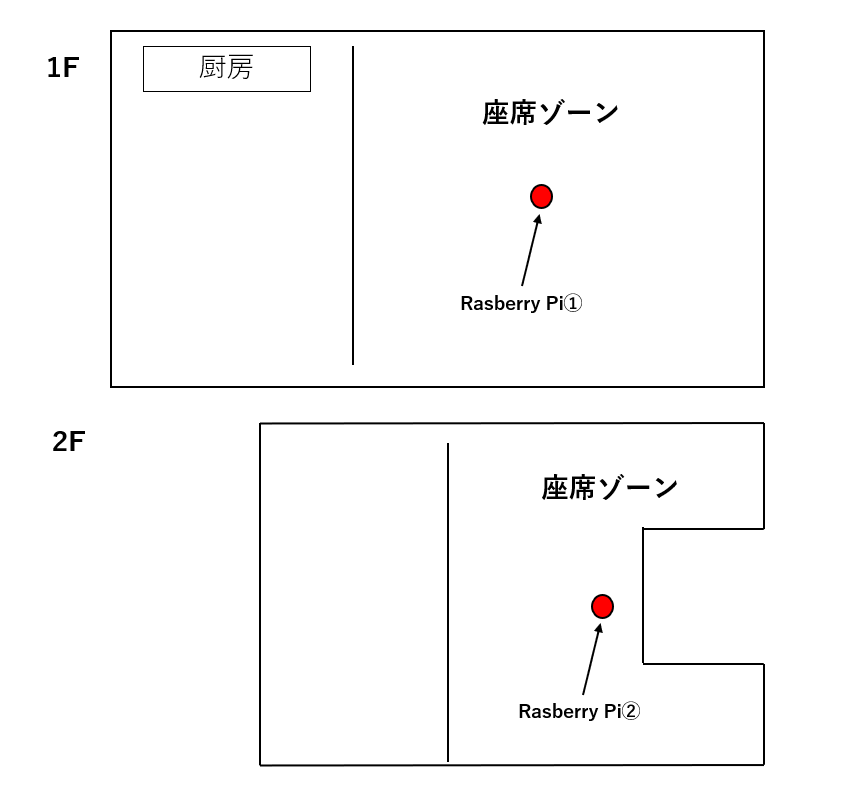
\includegraphics[scale=0.4]{./images/place_raspi.png}
  \centering
  \caption{学生食堂の概略図とRasberry Piの設置位置\label{raspi_place}}
\end{figure}

\subsubsection*{食堂利用人数の計測}
学生食堂の利用人数は,愛媛大学生協の方に提供していただいた決済データの時間情報と,
利用者が食堂を退出する際に返却されるトレーの数を計測し,算出する.
トレーの数の計測は2人体制で行い,返却場所にカメラを設置する.
計測者間で大きくズレが発生している場合は,カメラを確認し,再度計測する.
決済データは1分間隔で提供されるため,BLEスキャンデータと同様に1分間隔で食堂利用人数を算出する.

\subsection*{3.2 特徴量抽出}
本研究では,BLEスキャン情報から混雑度推定に有用な特徴量を抽出し,
モデルに入力することで混雑度を推定する.
基本的な特徴量は松田らの研究(文献)に基づき,表\ref{tbl:feastures}のように設計した.
本研究では,比較的大規模で開けた空間での混雑度推定を行う.
そのため障害物等による影響が少なく,RSSI値が比較的安定し,
Rasberry Piの位置から近ければ近いほどRSSI値が大きくなる事を考慮する.
このことから,RSSI値$S$に閾値を置き,$S$を変化させながら特徴量を算出することで,
各$S$の帯域毎に有益な特徴を抽出でき,混雑度推定の精度向上が期待できる.

\begin{table}[tb]
	\centering
	\caption{特徴量一覧}
	\label{tbl:feastures}
	\small
	\doublerulesep=0.3pt
    \begin{tabular}{l|p{5cm}} \hline\hline\hline
		特徴量名 & 内容 \\ \hline
		all\_num\_60\textsubscript{sec} & 過去 $T$ 秒間にスキャンされた,BD アドレスの総数\\ \hline
    unique\_num\_60\textsubscript{sec} & 過去 $T$ 秒間にスキャンされた,BD アドレスのユニーク数 \\ \hline
    unique\_ratio\_60\textsubscript{sec} & 過去 $T$ 秒間にスキャンされた,BD アドレスのうち,ユニークなデバイスの占める割合(ユニーク数 / 総数) \\ \hline
    unique\_num\_60\textsubscript{sec}\_Sdb & 過去 $T$ 秒間にスキャンされた,BD アドレスのうち,RSSI が閾値 Sdb より大きいもののユニーク数 \\ \hline\hline\hline
	\end{tabular}
\end{table}

\subsection*{3.3 混雑度推定モデル}
混雑度推定モデルは,BLEスキャン情報から抽出した特徴量を入力として,人数を出力するモデルである.
2.5項や2.6項で述べたようなモデルを用い,人数推定モデルを構築する.
詳しい学習の方法などは,A-4節で述べる.

\subsection*{3.4 評価指標}
本研究でモデルの性能評価に用いる指標について以下に述べる.

\subsubsection*{平均二乗誤差(Mean Squared Error, MSE)}
MSEは,予測値と実測値の差の二乗の平均を計算することにより,
モデルの誤差を定量化する指標である.数式で表すと,以下のようになる.
\begin{equation}
  \label{eq:mse}
  \mathrm{MSE} = \frac{1}{n} \sum_{i=1}^{n} (y_i - \hat{y}_i)^2
\end{equation}
ここで,$n$はサンプル数,$y_i$は実測値,$\hat{y}_i$は予測値である.

\subsubsection*{平均絶対誤差(Mean Absolute Error, MAE)}
MAEは,予測値と実測値の差の絶対値の平均を計算することにより,
モデルの誤差を定量化する指標である.数式で表すと,以下のようになる.
\begin{equation}
  \label{eq:mae}
  \mathrm{MAE} = \frac{1}{n} \sum_{i=1}^{n} |y_i - \hat{y}_i|
\end{equation}
ここで,$n$はサンプル数,$y_i$は実測値,$\hat{y}_i$は予測値である.

\subsubsection*{決定係数(Coefficient of Determination, $R^2$)}
決定係数は,予測値が実測値をどの程度説明できるかを示す指標である.  
数式で表すと,以下のようになる.
\begin{equation}
  \label{eq:r2}
  R^2 = 1 - \frac{\sum_{i=1}^{n} (y_i - \hat{y}_i)^2}{\sum_{i=1}^{n} (y_i - \bar{y})^2}
\end{equation}
ここで,$n$はサンプル数,$y_i$は実測値,$\hat{y}_i$は予測値,$\bar{y}$は実測値の平均である.